118. \begin{figure}[ht!]
\center{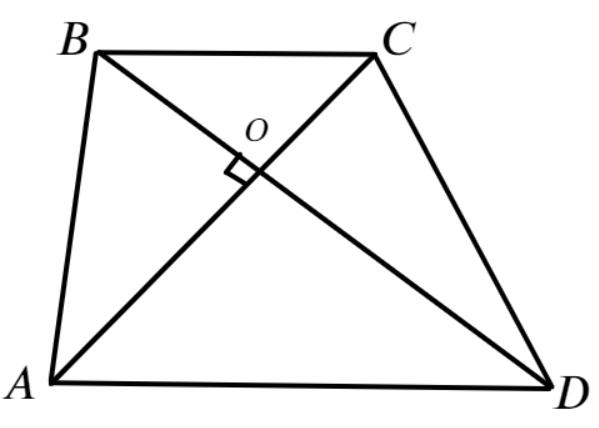
\includegraphics[scale=0.35]{g8-115.png}}
\end{figure}\\
Треугольники $AOB,\ BOC,\ COD$ и $AOD$ являются прямоугольными. Пусть $AO=x,\ CO=5-x,\ BO=y,\ DO=6-y.$ Тогда $S_{ABCD}=S_{\Delta AOB}+S_{\Delta BOC}+S_{\Delta COD}+S_{\Delta AOD}=\cfrac{xy}{2}+\cfrac{y(5-x)}{2}+\cfrac{(5-x)(6-y)}{2}+\cfrac{x(6-y)}{2}=\cfrac{xy+5y-xy+30-5y-6x+xy+6x-xy}{2}=15.$\\
